\section{Конструкторский раздел}

% NOTE:
% В конструкторском разделе описывается разрабатываемый метод
% В случае если в бакалаврском проекте разрабатывается новый метод или алгоритм, необходимо подробно изложить их суть, привести все необходимые для их реализации математические выкладки, обосновать последовательность этапов выполнения
% При этом для каждого этапа следует выделить необходимые исходные данные и получаемые результаты
% Для описания метода или алгоритма - Схема алгоритма
% В конце описания разработанного алгоритма должны быть приведены выбранные способы тестирования и сами тесты
% Перед формированием тестовых наборов данных целесообразно указать выделенные классы эквивалентности
% (тут же могут быть приведены выкладки по теоретическим рассчетам требуемой памяти и эффективности алгоритма; эти результаты могут быть использованы для обоснования правильности выбора метода из уже имеющихся альтернативных вариантов)
% Также должно быть приведено описание структуры разрабатываемого ПО, оно включает в себя:
% - описание общей структуры - определение основных частей (компонентов) и их взаимосвязей по управлению и по данным
% - декомпозицию компонентов и построение структурных иерархий
% - проектирование компонентов
% Для графического представления такого описания (если есть необходимость), следует использовать IDEF0 с декомпозицией исходной задачи на несколько уровней

% Рек. Объем 25-30 страниц

\subsection{Требования и ограничения метода}

Метод выделения составных частей научного текста на основе анализа распределения пикселей в сканирующей строке должен:
\begin{enumerate}
    \item Работать с одноколоночными Манхэттенскими макетами документов;
    \item Выделять текстовые блоки;
    \item Выделять таблицы;
    \item Выделять листинги;
    \item Выделять схемы алгоритмов;
    \item Выделять рисунки;
    \item Выделять графики;
    \item Работать на основе простых правил и эвристик, без использования нейросетей.
\end{enumerate}

% Разработать метод выделения ... строке
% Изложить особенности предложенного метода

\subsection{Описание разрабатываемого метода}

Поставленная задача решается в четыре этапа:
\begin{enumerate}
    \item Преобразование PDF документа в изображения;
    \item Первичная разметка страниц;
    \item Создание уточненной разметки на основе первичной;
    \item Объединение уточненной разметку в более крупные блоки.
\end{enumerate}

Разметка, ее уточнение и объединение происходят на основе определенных правил, которые будут описаны в данном разделе далее.

Основные этапы разрабатываемого метода представлены на IDEF0 диаграмме первого уровня (см. Рисунок \ref{fig:a1}).

\begin{figure}[H]
	\centering
	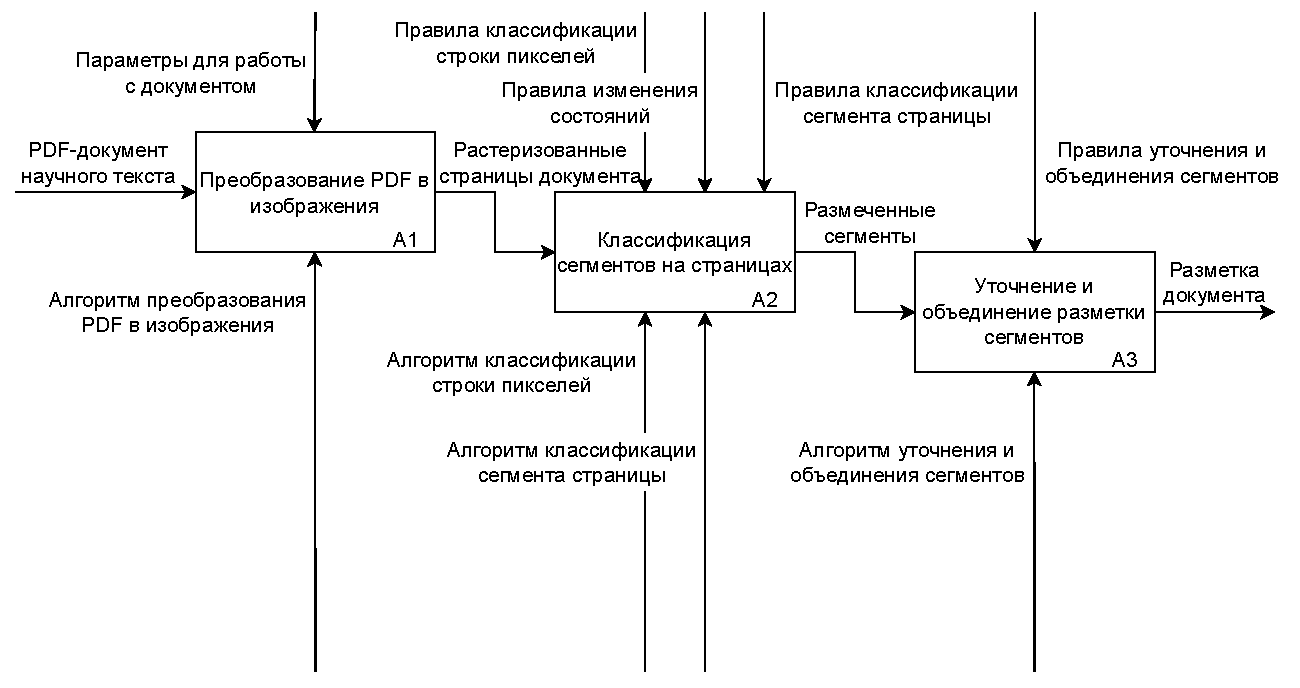
\includegraphics[width=\textwidth]{diag/a1-big.pdf}
	\caption{IDEF0-диаграмма метода выделения составных частей научного текста на основе анализа распределения пикселей в сканирующей строке}
	\label{fig:a1}
\end{figure}

\subsubsection{Первичная разметка}

Исходные данные --- изображение страницы документа.
Получаемый результат --- разметка страницы и информация о каждом сегменте на ней.

Разметка страницы --- массив кортежей типа
$$
(y\_start, y\_end, C),
$$
где $y\_start$ --- $y$-координата начала сегмента в пространстве изображения, $y\_end$ --- $y$-координата конца сегмента в пространстве изображения, $C$ --- класс сегмента, где $C \subseteq$ $\{$Фон, Немного текста, Много текста, Цвет, Черная линия средней длины, Длинная черная линия, Не определено$\}$.

Информация о сегменте содержит следующие данные:
\begin{enumerate}
    \item start --- ордината начала сегмента;
    \item end --- ордината конца сегмента;
    \item count\_long\_black\_line --- количество раз, когда при разметке сегмента встретилась строка, идентифицированная, как <<Длинная черная линия>>;
    \item count\_single\_long\_black\_line --- количество раз, когда при разметке сегмента встретилась строка, идентифицированная, как <<Длинная черная линия>>, считая несколько подряд идущих <<Длинных черных линий>> за одну;
    \item count\_medium\_black\_line --- количество раз, когда при разметке сегмента встретилась строка, идентифицированная, как <<Черная линия средней длины>>;
    \item count\_single\_medium\_black\_line --- количество раз, когда при разметке сегмента встретилась строка, идентифицированная, как <<Черная линия средней длины>>, считая несколько подряд идущих <<Черных линий средней длины>> за одну;
    \item count\_total\_medium\_black\_line --- количество раз, когда при разметке сегмента встретилась строка, идентифицированная, как <<Черная линия средней длины>>, с учетом всех <<Черных линий черной длины>> если таких было зафиксировано несколько внутри одной сканирующей строки;
    \item count\_many\_text --- количество раз, когда при разметке сегмента встретилась строка, идентифицированная, как <<Много текста>>;
    \item count\_few\_text --- количество раз, когда при разметке сегмента встретилась строка, идентифицированная, как <<Немного текста>>;
    \item count\_color --- количество раз, когда при разметке сегмента встретилась строка, идентифицированная, как <<Цвет>>;
    \item count\_undefined --- количество раз, когда при разметке сегмента встретилась строка, идентифицированная, как <<Не определено>>;
    \item count\_white\_px --- количество белых пикселей в сегменте;
    \item count\_color\_px --- количество цветных пикселей в сегменте;
    \item count\_gray\_px --- количество черных пикселей в сегменте (сумма трех данных счетчиков дает общее количество пикселей в сегменте);
    \item heatmap\_black --- массив, $i$-й элемент которого отражает количество черных пикселей в $i$-й колонке пикселей сегмента;
    \item heatmap\_color --- массив, $i$-й элемент которого отражает количество цветных пикселей в $i$-й колонке пикселей сегмента.
\end{enumerate}

Данная информация будет использоваться при уточнении разметки в следующем этапе.

\subsubsection{Уточненная разметка}

Исходные данные --- разметка страницы и информация о каждом сегменте на ней.
Получаемый результат --- уточненная разметка страницы.

Уточненная разметка страницы --- массив кортежей типа
$$
(y\_start, y\_end, C),
$$
где $y\_start$ --- $y$-координата начала сегмента в пространстве изображения, $y\_end$ --- $y$-координата конца сегмента в пространстве изображения, $C$ --- класс сегмента, где $C \subseteq$ $\{$Фон, Текст, Таблица, Листинг, Схема алгоритма, Рисунок, График, Не определено$\}$, причем координаты начала и конца сегментов совпадают с соответствующими координатами сегментов первичной разметки, уточняется только класс на основе информации о сегментах.

\subsubsection{Объединенная разметка}

Исходные данные --- уточненная разметка страницы.
Получаемый результат --- объединенная разметка страницы.

% При этом для каждого этапа следует выделить необходимые исходные данные и получаемые результаты

% Сформулировать и описать ключевые шаги метода в виде схем алгоритмов

% Разработать алгоритм, реализующий данный метод

\subsection{Тестирование и классы эквивалентности}

\subsection{Структура разрабатываемого ПО}

\subsection*{Вывод}
